\documentclass[a4paper]{article}
\usepackage{geometry}
\usepackage{graphicx}
\usepackage{natbib}
\usepackage{amsmath}
\usepackage{amssymb}
\usepackage{amsthm}
\usepackage{paralist}
\usepackage{epstopdf}
\usepackage{tabularx}
\usepackage{longtable}
\usepackage{multirow}
\usepackage{multicol}
\usepackage[hidelinks]{hyperref}
\usepackage{fancyvrb}
\usepackage{algorithm}
\usepackage{algorithmic}
\usepackage{float}
\usepackage{paralist}
\usepackage[svgname]{xcolor}
\usepackage{enumerate}
\usepackage{array}
\usepackage{times}
\usepackage{url}
\usepackage{fancyhdr}
\usepackage{comment}
\usepackage{environ}
\usepackage{times}
\usepackage{textcomp}
\usepackage{caption}
\usepackage{color}
\usepackage{xcolor}
\usepackage{subcaption}
\urlstyle{rm}

\setlength\parindent{0pt} % Removes all indentation from paragraphs
\theoremstyle{definition}
\newtheorem{definition}{Definition}[]
\newtheorem{conjecture}{Conjecture}[]
\newtheorem{example}{Example}[]
\newtheorem{theorem}{Theorem}[]
\newtheorem{lemma}{Lemma}
\newtheorem{proposition}{Proposition}
\newtheorem{corollary}{Corollary}

\floatname{algorithm}{Procedure}
\renewcommand{\algorithmicrequire}{\textbf{Input:}}
\renewcommand{\algorithmicensure}{\textbf{Output:}}
\newcommand{\abs}[1]{\lvert#1\rvert}
\newcommand{\norm}[1]{\lVert#1\rVert}
\newcommand{\RR}{\mathbb{R}}
\newcommand{\CC}{\mathbb{C}}
\newcommand{\Nat}{\mathbb{N}}
\newcommand{\br}[1]{\{#1\}}
\DeclareMathOperator*{\argmin}{arg\,min}
\DeclareMathOperator*{\argmax}{arg\,max}
\renewcommand{\qedsymbol}{$\blacksquare$}

\definecolor{dkgreen}{rgb}{0,0.6,0}
\definecolor{gray}{rgb}{0.5,0.5,0.5}
\definecolor{mauve}{rgb}{0.58,0,0.82}

\newcommand{\Var}{\mathrm{Var}}
\newcommand{\Cov}{\mathrm{Cov}}

\newcommand{\vc}[1]{\boldsymbol{#1}}
\newcommand{\xv}{\vc{x}}
\newcommand{\Sigmav}{\vc{\Sigma}}
\newcommand{\alphav}{\vc{\alpha}}
\newcommand{\muv}{\vc{\mu}}

\newcommand{\red}[1]{\textcolor{red}{#1}}

\def\x{\mathbf x}
\def\y{\mathbf y}
\def\w{\mathbf w}
\def\v{\mathbf v}
\def\E{\mathbb E}
\def\V{\mathbb V}

% TO SHOW SOLUTIONS, include following (else comment out):
\newenvironment{soln}{
    \leavevmode\color{blue}\ignorespaces
}{}


\hypersetup{
%    colorlinks,
    linkcolor={red!50!black},
    citecolor={blue!50!black},
    urlcolor={blue!80!black}
}

\geometry{
  top=1in,            % <-- you want to adjust this
  inner=1in,
  outer=1in,
  bottom=1in,
  headheight=3em,       % <-- and this
  headsep=2em,          % <-- and this
  footskip=3em,
}


\pagestyle{fancyplain}
\lhead{\fancyplain{}{Homework 2}}
\rhead{\fancyplain{}{CS 760 Machine Learning}}
\cfoot{\thepage}

\title{\textsc{Homework 2}} % Title

%%% NOTE:  Replace 'NAME HERE' etc., and delete any "\red{}" wrappers (so it won't show up as red)

\author{
Harry Zhang \\
hzhang699\\
GitHub Link: \url{}
} 

\date{}

\begin{document}

\maketitle 


\textbf{Instructions:} 
Use this latex file as a template to develop your homework. Submit your homework on time as a single pdf file to Canvas. Please wrap your code and upload to a public GitHub repo, then attach the link below the instructions so that we can access it. You can choose any programming language (i.e. python, R, or MATLAB), as long as you implement the algorithm from scratch (e.g. do not use sklearn on questions 1 to 7 in section 2). Please check Piazza for updates about the homework.

\section{A Simplified Decision Tree}
You are to implement a decision-tree learner for classification.
To simplify your work, this will not be a general purpose decision tree.  Instead, your program can assume that
\begin{itemize}
\item each item has two continuous features $\x \in \RR^2$
\item the class label is binary and encoded as $y \in \{0,1\}$
\item data files are in plaintext with one labeled item per line, separated by whitespace:
$$x_{11} \quad x_{12} \quad y_1$$
$$...$$
$$x_{n1} \quad x_{n2} \quad y_n$$
\end{itemize}

Your program should implement a decision tree learner according to the following guidelines:
\begin{itemize}
\item Candidate splits $(j,c)$ for numeric features should use a threshold $c$ in feature dimension $j$ in the form of $x_{j}\ge c$.
\item $c$ should be on values of that dimension present in the training data; i.e. the threshold is on training points, not in between training points. You may enumerate all features, and for each feature, use all possible values for that dimension.
\item You may skip those candidate splits with zero split information (i.e. the entropy of the split), and continue the enumeration.
\item The left branch of such a split is the ``then'' branch, and the right branch is ``else''.
\item Splits should be chosen using information gain ratio. If there is a tie you may break it arbitrarily.
\item The stopping criteria (for making a node into a leaf) are that 
	\begin{itemize}
	\item the node is empty, or
	\item all splits have zero gain ratio (if the entropy of the split is non-zero), or
	\item the entropy of any candidates split is zero
	\end{itemize}
\item To simplify, whenever there is no majority class in a leaf, let it predict $y=1$.
\end{itemize}

\section{Questions}
\begin{enumerate}
\item (Our algorithm stops at pure labels) [10 pts] If a node is not empty but contains training items with the same label, why is it guaranteed to become a leaf?  Explain. You may assume that the feature values of these items are not all the same. \\
\begin{soln}
If a node is not empty but contains training items with the same label, it is guaranteed to become a leaf because the entropy of the split is zero. The entropy of the split is zero because the entropy of the split is defined as $H(S) = -\sum_{i=1}^{c} p_i \log_2 p_i$, where $p_i$ is the probability of the $i$th class. Since all the training items in the node have the same label, the entropy of the split is zero because $p_i = 1$ for some $i$.
\end{soln}
\item (Our algorithm is greedy)  [10 pts] Handcraft a small training set where both classes are present but the algorithm refuses to split; instead it makes the root a leaf and stop;
Importantly, if we were to manually force a split, the algorithm will happily continue splitting the data set further and produce a deeper tree with zero training error.
You should (1) plot your training set, (2) explain why.  Hint: you don't need more than a handful of items. \\

\begin{soln}
  \begin{figure}
    \centering
    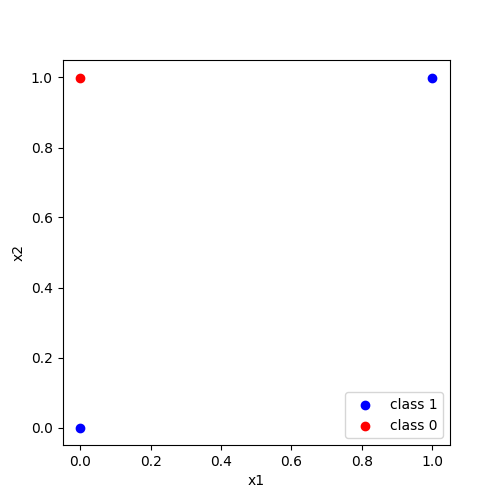
\includegraphics[width=0.5\textwidth]{./data/p2q2.png}
    \caption{The training set where both classes are present but the algorithm refuses to split}
    \label{fig:q2}
  \end{figure}
  See Figure~\ref{fig:q2}, in this case we can't draw boundary between class 0 and 1 because the closest value in either dimension is one unit of increment, and we need to make sure split is on training points, not in between training points. Therefore, the algorithm refuses to split.
\end{soln}

\item (Information gain ratio exercise)  [10 pts] Use the training set Druns.txt.  For the root node, list all candidate cuts and their information gain ratio. If the entropy of the candidate split is zero, please list its mutual information (i.e. information gain). Hint: to get $\log_2(x)$ when your programming language may be using a different base, use \verb|log(x)/log(2)|. Also, please follow the split rule in the first section. \\
\begin{soln}
  In the root node: all the candidate cuts are following (followed by rule (j,c) j is feature and c is threshold): \\
  (0, 0.0), (0, 0.1), (1, -2.0), (1, -1.0), (1, 0.0), (1, 1.0), (1, 2.0), (1, 3.0), (1, 4.0), (1, 5.0), (1, 6.0), (1, 7.0), (1, 8.0) \\
  The information gain ratio for each candidate cut is following: \\
  (0, 0.0): zero split entropy \\
  (0, 0.1):  0.10051807676021828\\
  (1, -2.0): zero split entropy \\
  (1, -1.0): 0.10051807676021828 \\
  (1, 0.0): 0.0559537596312636 \\
  (1, 1.0): 0.00578004220515232 \\
  (1, 2.0): 0.0011443495172767494 \\
  (1, 3.0): 0.016411136842102134 \\
  (1, 4.0): 0.04974906418177849 \\
  (1, 5.0): 0.11124029586339806 \\
  (1, 6.0): 0.23609960614360798 \\
  (1, 7.0): 0.055953759631263686 \\
  (1, 8.0): 0.4301569161309807 \\
\end{soln}
\item (The king of interpretability)  [10 pts] Decision tree is not the most accurate classifier in general.  However, it persists.  This is largely due to its rumored interpretability: a data scientist can easily explain a tree to a non-data scientist.  Build a tree from D3leaves.txt.  Then manually convert your tree to a set of logic rules.  Show the tree\footnote{When we say show the tree, we mean either the standard computer science tree view, or some crude plaintext representation of the tree -- as long as you explain the format.  When we say visualize the tree, we mean a plot in the 2D $\x$ space that shows how the tree will classify any points.} and the rules. \\
\begin{soln}
  \begin{figure}
    \begin{subfigure}{.5\textwidth}
      \centering
      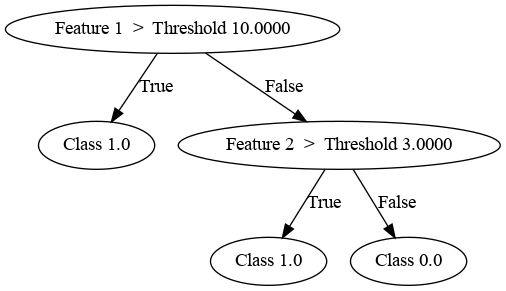
\includegraphics[width=0.8\linewidth]{./data/custom_decision_tree_D3leaves.png}
      \caption{Decision Tree for D3leaves.txt}
      \label{fig:decision_treeD3leaves}
    \end{subfigure}
    \begin{subfigure}{.5\textwidth}
      \centering
      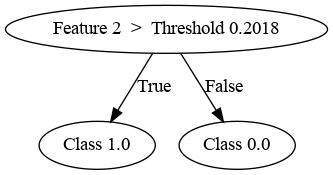
\includegraphics[width=0.8\linewidth]{./data/custom_decision_tree_D1.png}
      \caption{Decision Tree for D1.txt}
      \label{fig:decision_tree_d1}
    \end{subfigure}
    \caption{Decision Tree}
  \end{figure}
  For decision tree, see the Figure~\ref{fig:decision_treeD3leaves}. 
\end{soln}

\item (Or is it?)  [10 pts] For this question only, make sure you DO NOT VISUALIZE the data sets or plot your tree's decision boundary in the 2D $\x$ space.  If your code does that, turn it off before proceeding.  This is because you want to see your own reaction when trying to interpret a tree.  You will get points no matter what your interpretation is.
And we will ask you to visualize them in the next question anyway.
  \begin{itemize}
  
  \item Build a decision tree on D1.txt.  Show it to us in any format (e.g. could be a standard binary tree with nodes and arrows, and denote the rule at each leaf node; or as simple as plaintext output where each line represents a node with appropriate line number pointers to child nodes; whatever is convenient for you). Again, do not visualize the data set or the tree in the $\x$ input space.  In real tasks you will not be able to visualize the whole high dimensional input space anyway, so we don't want you to ``cheat'' here. 
  \begin{soln}
    % \begin{figure}
    %   \centering
    %   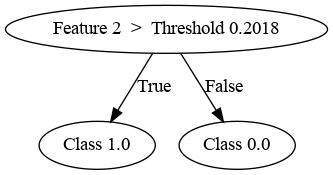
\includegraphics[width=0.4\textwidth]{./data/custom_decision_tree_D1.png}
    %   \caption{Decision Tree for D1.txt}
    %   \label{fig:decision_tree_d1}
    % \end{figure}
    See the Figure~\ref{fig:decision_tree_d1} for decision tree trained on dataset D1.txt. So the logic is simple as following: for given input $\x =[x_1 \;\; x_2]^T$, if $x_2 > 0.2018$, then the predicted label is 1, otherwise, the predicted label is 0.
  \end{soln}
  \item Look at your tree in the above format (remember, you should not visualize the 2D dataset or your tree's decision boundary) and try to interpret the decision boundary in human understandable English. 
  \begin{soln}
    See the Figure~\ref{fig:decision_tree_d1} for decision tree trained on dataset D1.txt.
  \end{soln}
  \item Build a decision tree on D2.txt.  Show it to us. 
  \begin{soln}
    \begin{figure}
      \centering
      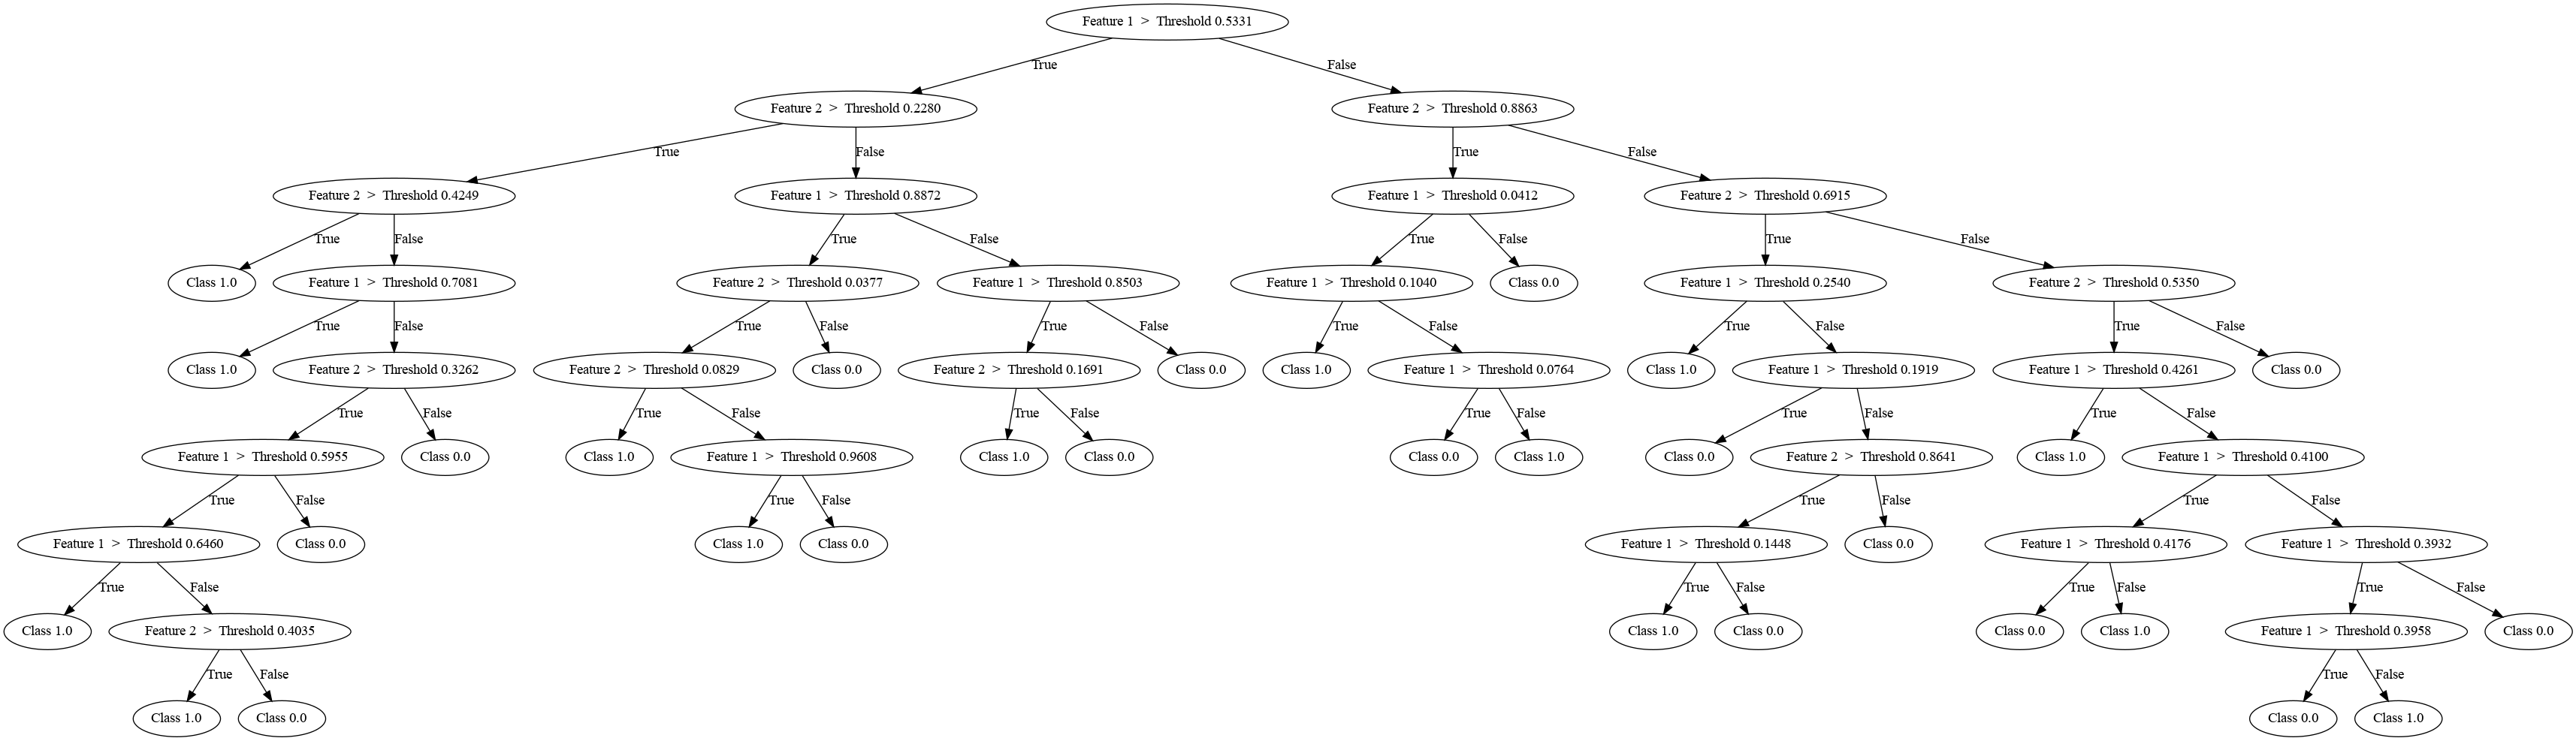
\includegraphics[width=0.9\textwidth]{./data/custom_decision_tree_D2.png}
      \caption{Decision Tree for D2.txt}
      \label{fig:decision_tree_d2}
    \end{figure}
    \\See the Figure~\ref{fig:decision_tree_d2} for decision tree trained on dataset D2.txt.
  \end{soln}
  \item Try to interpret your D2 decision tree. Is it easy or possible to do so without visualization? \\
  \begin{soln}
    It is not easy to interpret this decision tree, because as shown in Figure~\ref{fig:decision_tree_d2}, the decision tree is very deep and the logic is very complicated.
  \end{soln}
  \end{itemize}

\item (Hypothesis space)  [10 pts] For D1.txt and D2.txt, do the following separately:
  \begin{itemize}
  
  \item Produce a scatter plot of the data set.
    \begin{soln}
      \begin{figure}
        \centering
        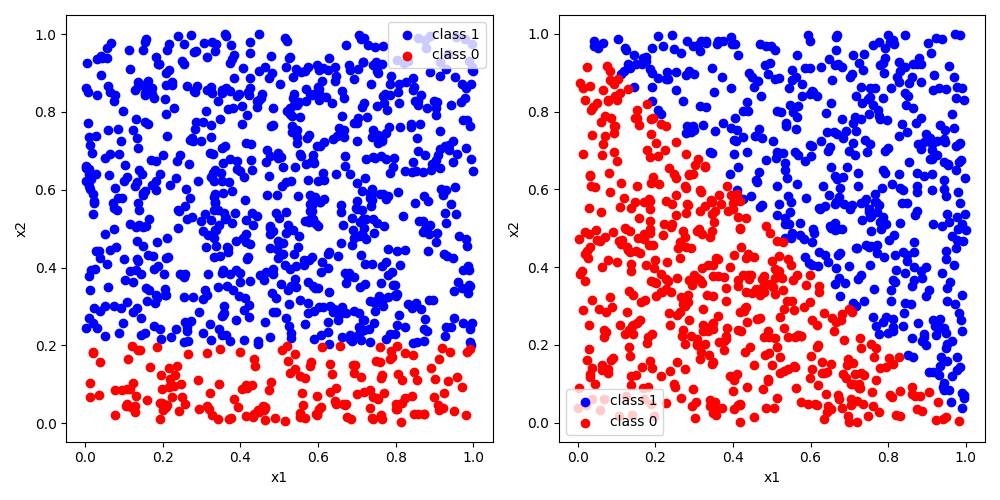
\includegraphics[width=0.9\textwidth]{./data/p2q5.png}
        \caption{scatter plot for D1 and D2: right is D1, left is D2}
        \label{fig:scatterD1D2}
      \end{figure}
      \\See the Figure~\ref{fig:scatterD1D2} for scatter plot of D1 and D2.
    \end{soln}
  \item Visualize your decision tree's decision boundary (or decision region, or some other ways to clearly visualize how your decision tree will make decisions in the feature space).
  \begin{soln}
    \begin{figure}
      \begin{subfigure}{.6\textwidth}
        % \centering
        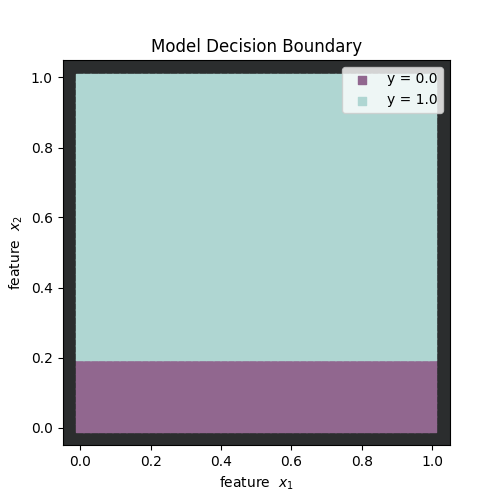
\includegraphics[width=0.9\linewidth]{./data/d1bound.png}
        \caption{Decision Tree Boundary for D1.txt}
        \label{fig:db1}
      \end{subfigure}
      \begin{subfigure}{.6\textwidth}
        %\centering
        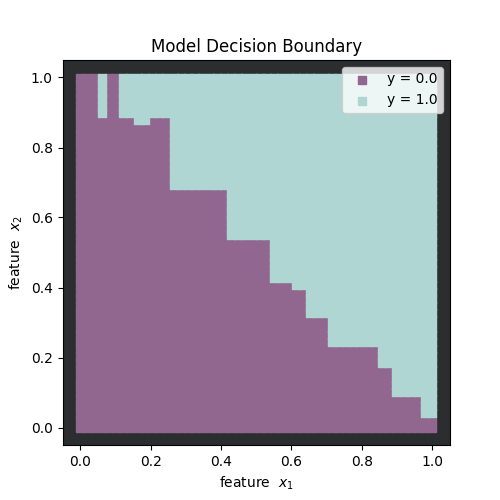
\includegraphics[width=0.9\linewidth]{./data/d2bound.png}
        \caption{Decision Tree Boundary for D2.txt}
        \label{fig:db2}
      \end{subfigure}
      \caption{Decision Tree}
    \end{figure}
    \\See the Figure~\ref{fig:db1} and Figure~\ref{fig:db2} for decision tree boundary for D1 and D2.
  \end{soln}
  \end{itemize}
Then discuss why the size of your decision trees on D1 and D2 differ.  Relate this to the hypothesis space of our decision tree algorithm. \\
\begin{soln}
  The size of decision tree on D1 is much smaller than D2's. This is because we are doing binary classification, and the distribution of D1 is much simpler than D2's, because D1 dataset divided through a horizontal line, but D2 divided through diagonal lines that requires many of vertical and horizontal boundary to approximate. So the data space of D1 is much smaller than D2's.
\end{soln}
\item (Learning curve)  [20 pts] We provide a data set Dbig.txt with 10000 labeled items.  Caution: Dbig.txt is sorted.
  \begin{itemize}
  
  \item You will randomly split Dbig.txt into a candidate training set of 8192 items and a test set (the rest).  Do this by generating a random permutation, and split at 8192.
  
  \item Generate a sequence of five nested training sets $D_{32} \subset D_{128} \subset D_{512} \subset D_{2048} \subset D_{8192}$ from the candidate training set.  The subscript $n$ in $D_n$ denotes training set size.  The easiest way is to take the first $n$ items from the (same) permutation above.  This sequence simulates the real world situation where you obtain more and more training data.
  
  \item For each $D_n$ above, train a decision tree.  Measure its test set error $err_n$.  Show three things in your answer: (1) List $n$, number of nodes in that tree, $err_n$. (2) Plot $n$ vs. $err_n$.  This is known as a learning curve (a single plot). (3) Visualize your decision trees' decision boundary (five plots). \\
  \end{itemize}
  \begin{soln}
    \\For (1), see the Table~\ref{tab:errn} for $n$, number of nodes in that tree, $err_n$.
    \begin{table}
      \centering
      \begin{tabular}{|c|c|c|}
        \hline
        n & number of nodes & $err_n$ \\
        \hline
        32 & 1 & 0.409 \\
        \hline
        128 & 9 & 0.139 \\
        \hline
        512 & 35 & 0.067 \\
        \hline
        2048 & 45 & 0.091 \\
        \hline
        8192 & 213 & 0.020 \\
        \hline
      \end{tabular}
      \caption{This table has information about data size: $n$, number of nodes in that tree, and error rate: $err_n$}
      \label{tab:errn}
    \end{table}
    \\For (2), see the Figure~\ref{fig:errn} for $n$ vs. $err_n$.
    \begin{figure}
      \centering
      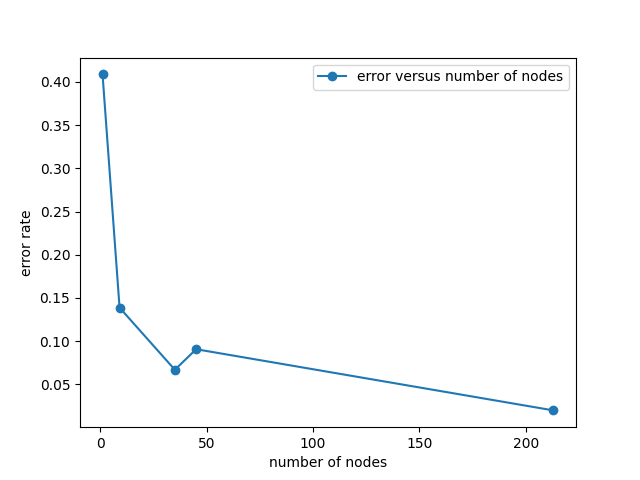
\includegraphics[width=0.5\textwidth]{./data/errvsnodes.png}
      \caption{This figure shows the relationship between number of nodes and $err_n$}
      \label{fig:errn}
    \end{figure}
    \\For (3), see the Figure~\ref{fig:db32}, Figure~\ref{fig:db128}, Figure~\ref{fig:db512}, Figure~\ref{fig:db2048}, Figure~\ref{fig:db8192} for decision tree boundary for $D_{32}, D_{128}, D_{512}, D_{2048}, D_{8192}$.
    \begin{figure}
      \centering
      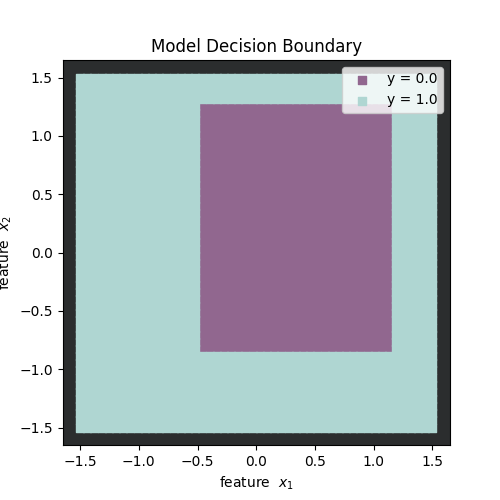
\includegraphics[width=0.2\textwidth]{./data/db32.png}
      \caption{Decision Tree Boundary for D32.txt}
      \label{fig:db32}
    \end{figure}
    \begin{figure}
      \centering
      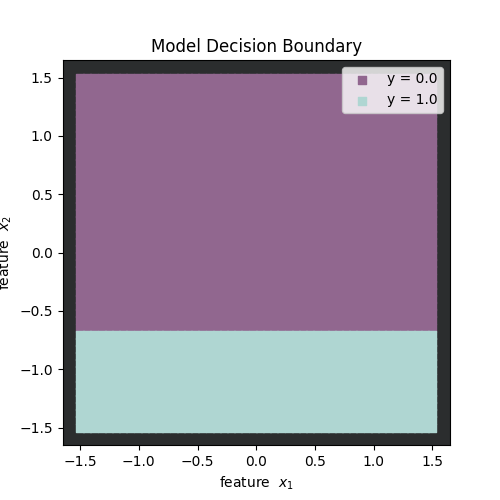
\includegraphics[width=0.2\textwidth]{./data/db128.png}
      \caption{Decision Tree Boundary for D128.txt}
      \label{fig:db128}
    \end{figure}
    \begin{figure}
      \centering
      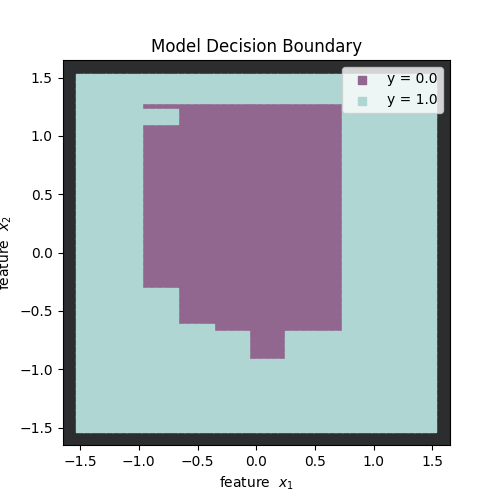
\includegraphics[width=0.2\textwidth]{./data/db512.png}
      \caption{Decision Tree Boundary for D512.txt}
      \label{fig:db512}
    \end{figure}
    \begin{figure}
      \centering
      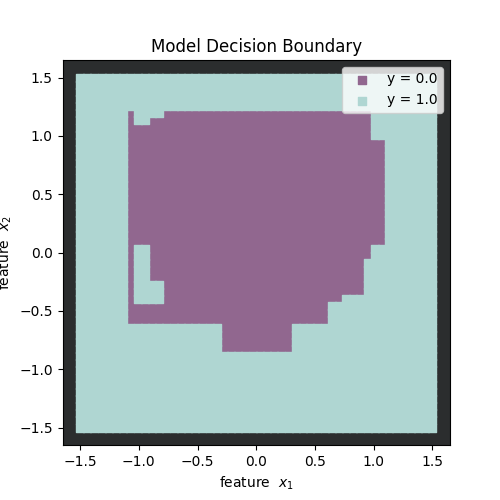
\includegraphics[width=0.2\textwidth]{./data/db2048.png}
      \caption{Decision Tree Boundary for D2048.txt}
      \label{fig:db2048}
    \end{figure}
    \begin{figure}
      \centering
      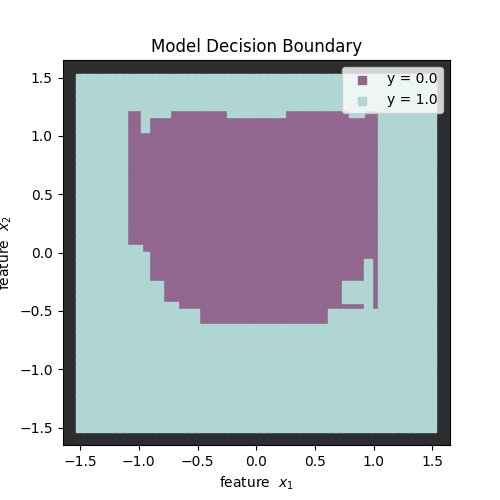
\includegraphics[width=0.2\textwidth]{./data/db8192.png}
      \caption{Decision Tree Boundary for D8192.txt}
      \label{fig:db8192}
    \end{figure}
  \end{soln}
\end{enumerate}

\section{sklearn [10 pts]}
Learn to use sklearn (\url{https://scikit-learn.org/stable/}).
Use sklearn.tree.DecisionTreeClassifier to produce trees for datasets $D_{32}, D_{128}, D_{512}, D_{2048}, D_{8192}$.  Show two things in your answer: (1) List $n$, number of nodes in that tree, $err_n$. (2) Plot $n$ vs. $err_n$.
\begin{soln}
  \\1. See the Table~\ref{tab:errnsk} for $n$, number of nodes in that tree, $err_n$.
  \begin{table}
    \centering
    \begin{tabular}{|c|c|c|}
      \hline
      n & number of nodes & $err_n$ \\
      \hline
      32 & 9 & 0.19999999999999996 \\
      \hline
      128 & 23 & 0.17948717948717952 \\
      \hline
      512 & 43 & 0.045454545454545414 \\
      \hline
      2048 & 85 & 0.03252032520325199 \\
      \hline
      8192 & 231 & 0.017900732302685074 \\
      \hline
    \end{tabular}
    \caption{This table has information about data size: $n$, number of nodes in that tree, and error rate: $err_n$}
    \label{tab:errnsk}
  \end{table}
  \\2. See the Figure~\ref{fig:errnsk} for $n$ vs. $err_n$.
  \begin{figure}
    \centering
    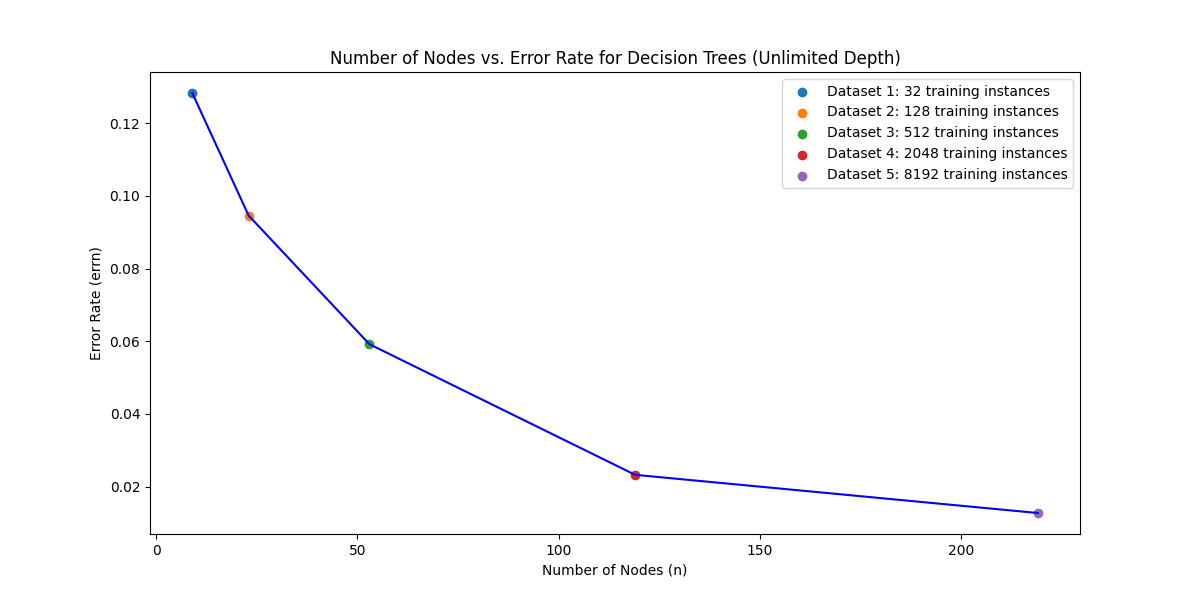
\includegraphics[width=0.5\textwidth]{./data/p3.png}
    \caption{This figure shows the relationship between number of nodes and $err_n$}
    \label{fig:errnsk}
  \end{figure}
\end{soln}
\section{Lagrange Interpolation [10 pts]}
Fix some interval $[a, b]$ and sample $n = 100$ points $x$ from this interval uniformly. Use these to build a training set consisting of $n$ pairs $(x, y)$ by setting function $y = sin(x)$. \\

Build a model $f$ by using Lagrange interpolation, check more details in \url{https://en.wikipedia.org/wiki/Lagrange_polynomial} and \url{https://docs.scipy.org/doc/scipy/reference/generated/scipy.interpolate.lagrange.html}. \\

Generate a test set using the same distribution as your test set. Compute and report the resulting model’s train and test error. What do you observe?
Repeat the experiment with zero-mean Gaussian noise $\epsilon$ added to $x$. Vary the standard deviation for $\epsilon$ and report your findings.
\begin{soln}
  \\See Figure~\ref{fig:lagrange} for the result of Lagrange interpolation error rate v.s. amount of noise added. Error is calculated by log mean square error.
  \begin{figure}
    \centering
    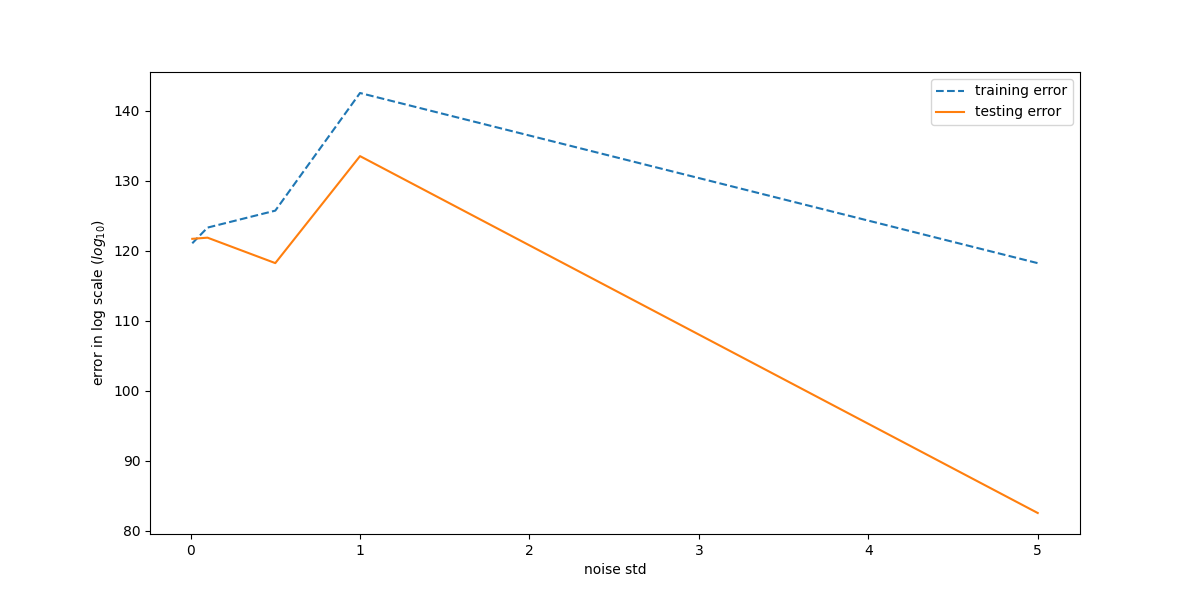
\includegraphics[width=0.7\textwidth]{./data/p4.png}
    \caption{This figure shows the result of Lagrange interpolation}
    \label{fig:lagrange}
  \end{figure}
\end{soln}
\bibliographystyle{apalike}
\end{document}
